\section{Teorema de Cauchy e Aplicaciones}

\hypertarget{thm11}{}
\parbox[a]{0.7\linewidth}{
\begin{theorem}
    \textbf{1.1. (\emph{Goursat})} Sean \(f\in \ho(\Omega) \) e \(T\subset \Omega \) un triángulo cuyo borde e interior están contenidos en \(\Omega\), entonces 
    \[\int_T f(z) \ dz = 0. \]
\end{theorem}
}

\comentario{No admite resumen, pero se trata de un argumento de bisección, véase \cite[pag. 34]{stein}}

\begin{corollary}
    \textbf{1.2.} Lo enunciado en \(\blacksquare\) \hyperlink{thm11}{1.1. (\emph{Goursat})} vale tambien para rectágulos.
\end{corollary}

\hypertarget{thm221}{}
\begin{theorem}
    \textbf{2.1.} Sean \(D := B(z_0;r)\) e \(f\in \ho(D)\), entonces existe primitiva de \(f\) en \(D\). \comentario{No admite resumen, véase \cite[pag. 37]{stein}} 
\end{theorem}

\hypertarget{thm222}{}
\begin{theorem}
    \textbf{2.2. (\emph{Cauchy en el disco})} Si \(f\in \ho(D)\), entonces 
    \[\displaystyle \int_\gamma f(z) \ dz = 0 \ : \ \gamma  \subset D \text{ es curva cerrada}. \ \textcolor{gray}{\rightarrow \blacksquare \ \hyperlink{thm221}{2.1.} \text{\ + \ \scriptsize $\boxtimes$}\  \hyperlink{coro133}{3.3.}}\] 
\end{theorem}

%\demo{Por el \(f\) tiene primitiva, luego el resultado sigue del .}

\vspace{-0.5cm}
\begin{corollary}
    \textbf{2.3.} Si  \ \(f\in \ho(\Omega)\) e \(\overline{D} \subset \Omega \), entonces \(\displaystyle\int_{\partial D} f(z) \ dz\). 
\end{corollary}

\begin{textblock*}{6cm}(12.8cm, 9.7cm)
        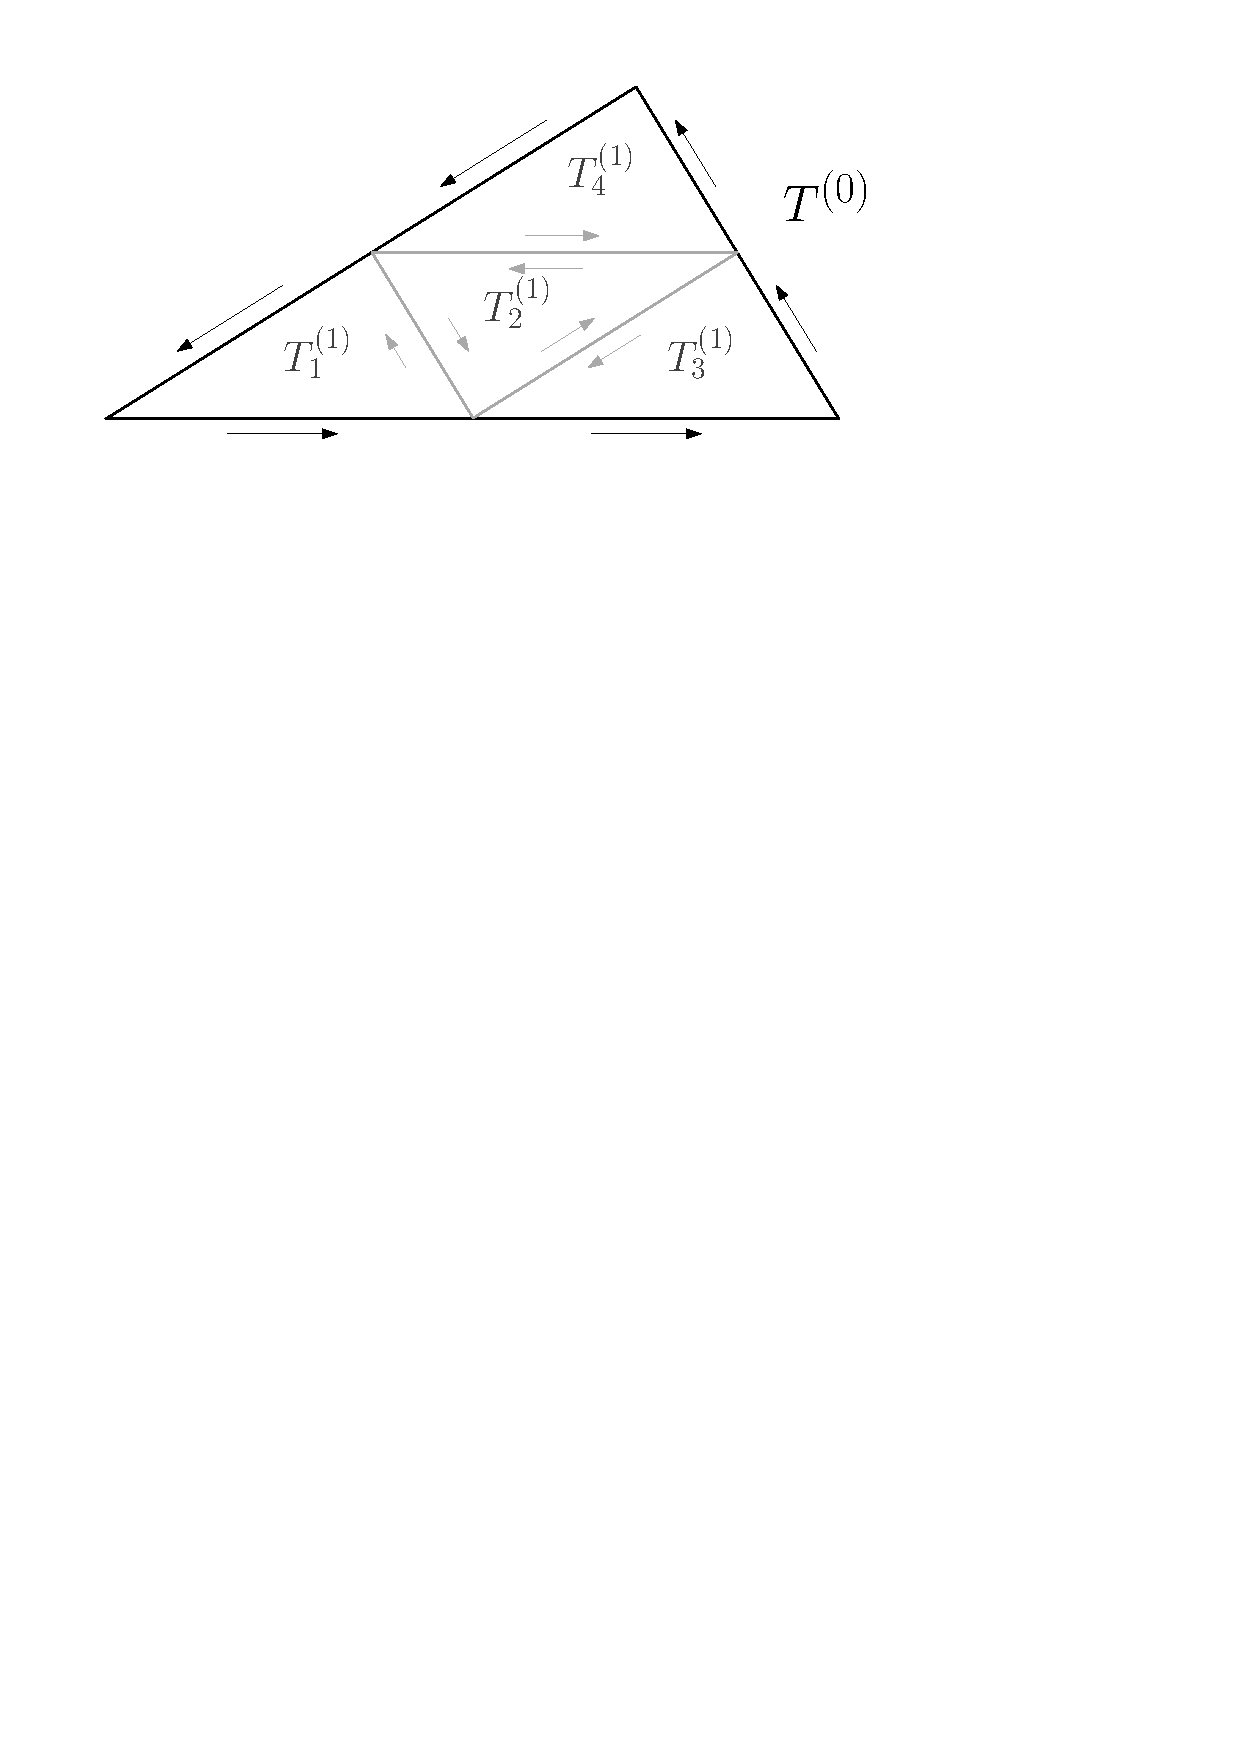
\includegraphics[width = \linewidth]{Imagens/T.pdf}
\end{textblock*}

\begin{textblock*}{5cm}(13.5cm, 21.7cm)
        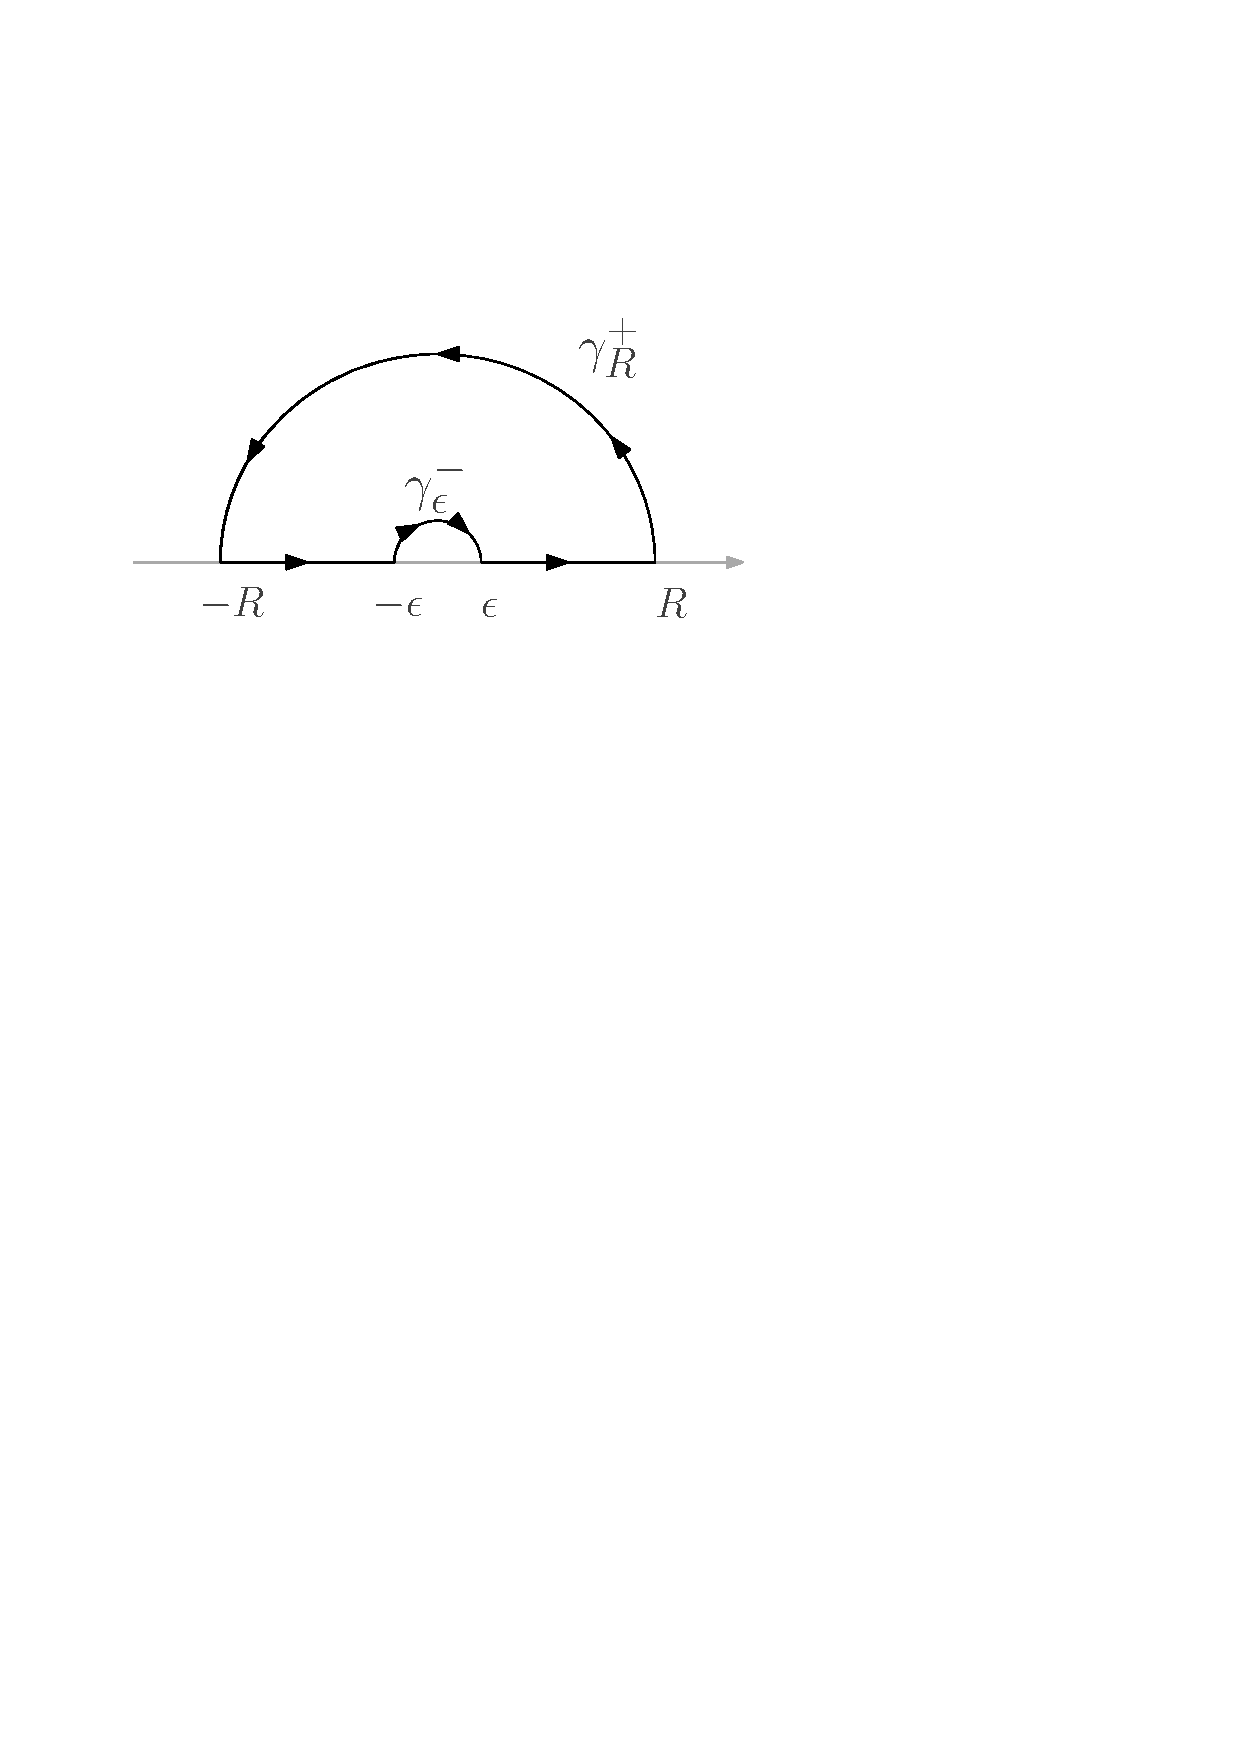
\includegraphics[width = \linewidth]{Imagens/ExInt.pdf}
\end{textblock*}


\ejemplo{
    \centering Motivación detrás del Teorema
    \tcblower
    %\parbox[a]{0.3\linewidth}{\- }
    \parbox[b]{0.7\linewidth}{
    \begin{example}
        Calcule usando \(\blacksquare\) \hyperlink{thm222}{2.2.}, haciendo  \(\epsilon \to 0\), 
        \[\displaystyle \textcolor{gray}{\frac{\pi}{2}=}  \int_\epsilon^{\nicefrac{1}{\epsilon}} \frac{1- \cos x}{x^2} \ dx \ \ \textcolor{gray}{\sim f(z) = \frac{1 - e^{iz}}{z^2}}.\]  
    \end{example}
    }
}

\subsection*{Formúla integral de Cauchy}

\vspace{-0.7cm}
\hypertarget{thm241}{}
%\parbox[a]{0.7\linewidth}{
\begin{theorem}
    \textbf{4.1.} Si \(f\in \ho(\Omega)\) e \(\overline{D}\subset \Omega\), entonces 
    \(\displaystyle f(z) = \frac{1}{2\pi i } \int_{\partial D} \overset{\textcolor{gray}{\underset{\uparrow }{F(\zeta)}}}{\frac{f(\zeta)}{\zeta - z}} \ d\zeta, \  \ z \in D \).
\end{theorem}
%}

%\parbox{0.75\linewidth}{
\demo{ %\footnotesize 
        \[0 =  \lim_{\epsilon \to 0} \int_{\Gamma_{\delta, \epsilon}} F(\zeta) \ d\zeta = \int_{\partial D} F(\zeta ) \ d\zeta + I_\epsilon  + \int_{\partial D_\epsilon} \frac{f(z)}{\zeta - z} \ d\zeta. \hspace{4cm}\]
        \hrule width 13cm 
        \vspace{0.3cm}
        \textcolor{gray}{\[I_\epsilon = \int_{\partial D_\epsilon} \frac{f(\zeta) - f(z)}{\zeta - z} \ d\zeta \to 0 \text{ \ e \ }\int_{\partial D_\epsilon} \frac{f(z)}{\zeta - z} \ d\zeta = - f(z) 2\pi i.\hspace{4cm}\]} 
        \vspace{-0.2cm}
}
%}

\hypertarget{coro242}{}
\begin{corollary}
    \textbf{4.2. (\emph{Formúla integral de Cauchy})} Si \( f\in \ho(\Omega)\), entonces \(f\) tiene derivadas complejas de todos los ordenes en \(\Omega\). Más aún, si \(\overline{D}\subset \Omega \), entonces 
    \[f^{(n)}(z) = \frac{n!}{2\pi i } \int_{\partial D} \frac{f(\zeta)}{\zeta - z} \ d\zeta, \ \ z \in D.\]
\end{corollary}

\demo{ 
    Por inducción, escriba \(f^{(n)}(z) = \underset{h\to 0}{\lim} (\cdots) \) usando \(\blacksquare\) \hyperlink{thm241}{4.1.} para expresar \(f^{(n-1)}(z)\), luego use \(A^n -B^n = (A-B) [A^{n-1} + A^{n-2}B + \cdots + B^{n-1}]\) para simplificar.
    % \[\lim_{h\to 0}\frac{f^{(n-1)} (z+h) - f^{(n-1)}(z)}{h} = \]
}

\begin{textblock*}{5cm}(15.7cm, 2.6cm)
        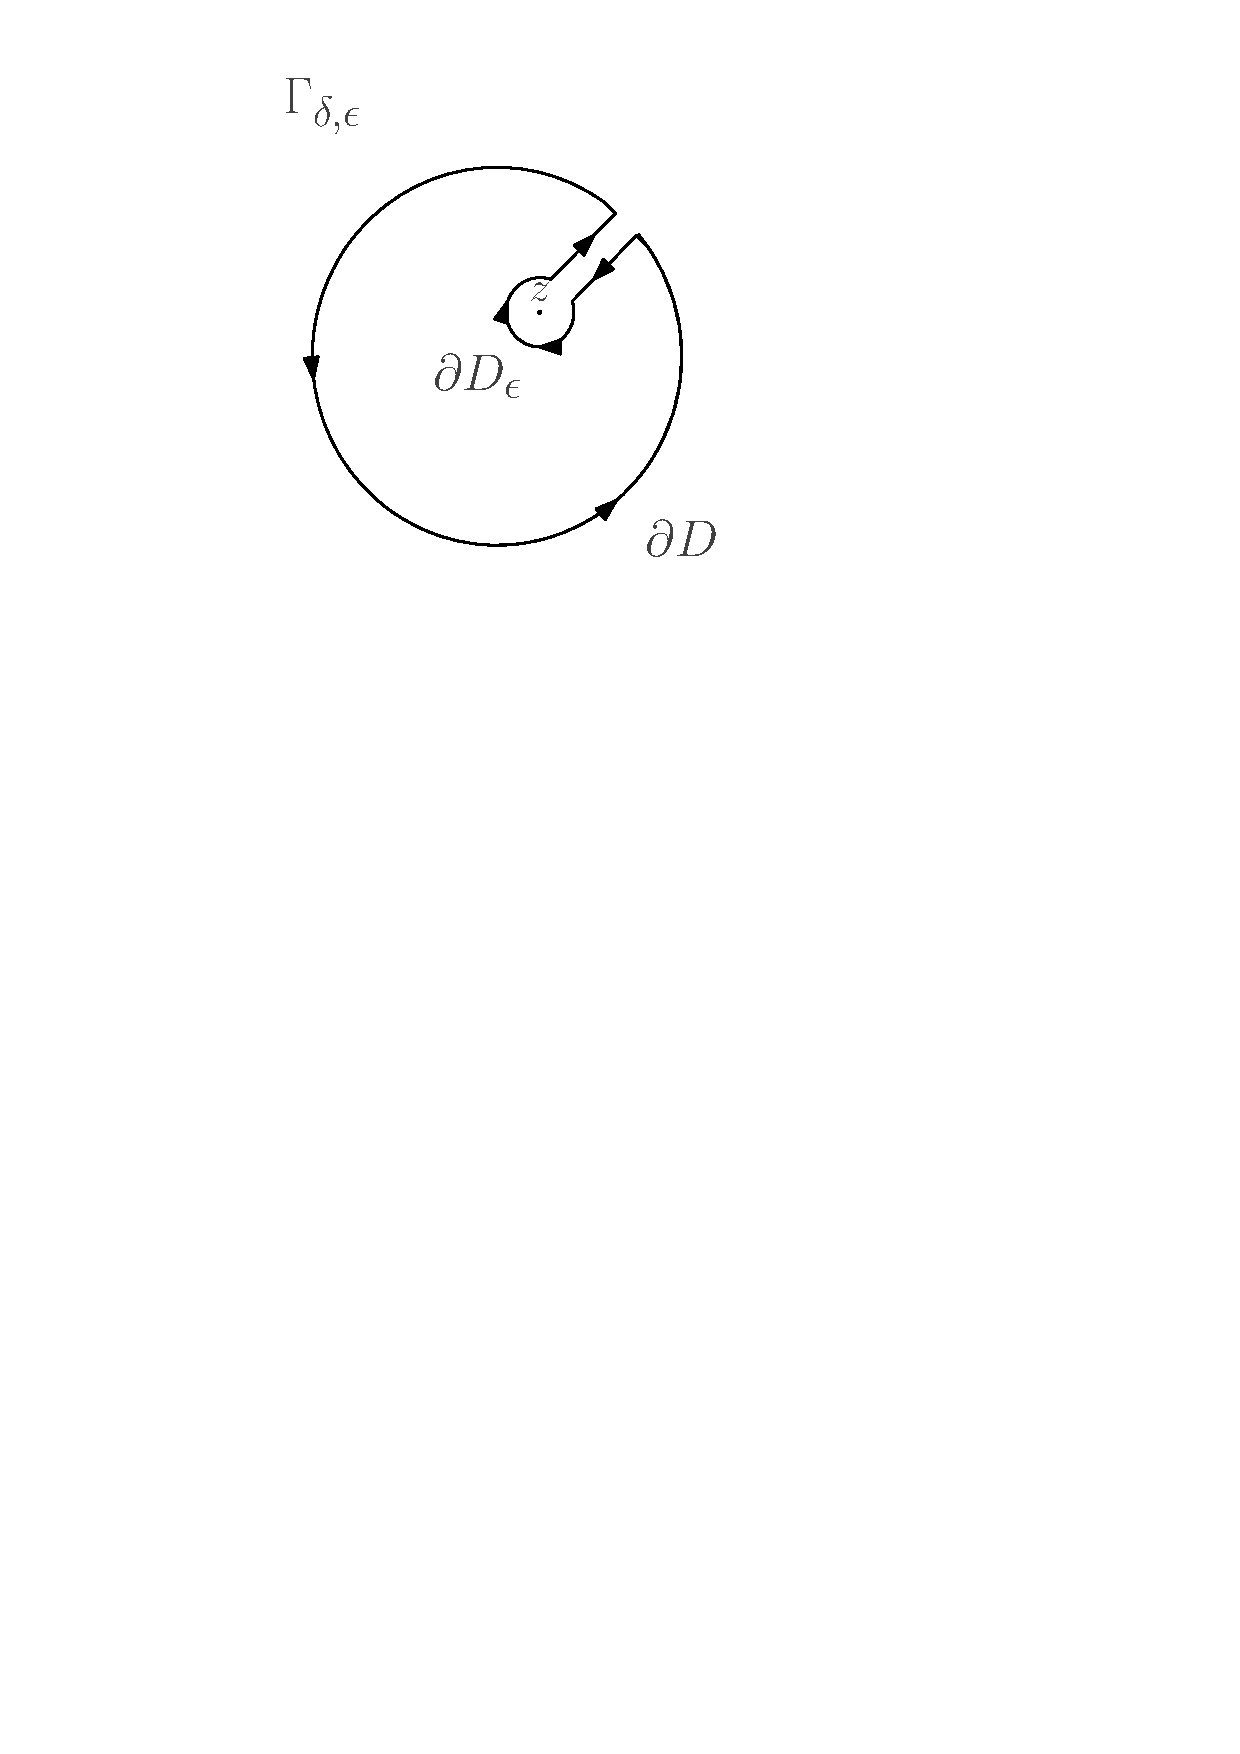
\includegraphics[width = 0.6\linewidth]{Imagens/Cauchy.pdf}
\end{textblock*}

\hypertarget{coro243}{}
\begin{corollary}
    \textbf{4.3. (\emph{Desigualdad de Cauchy})}  Si \( f\in \ho(\Omega)\) e \(B[z_0;R] \subset \Omega \), then 
    \[|f^{(n)}(z_0)|\leq \frac{n! \|f\|_{\partial D}}{R^n}, \text{ donde } \|f\|_{\partial D}:= \sup_{\partial D} |f(z)|\]
\end{corollary}

\demo{  
    \[|f^{(n)}(z_0) | = \frac{n!}{2\pi} \left| \int_{\partial D} \frac{f(\zeta )}{\zeta - z} \ d \zeta \right| = \frac{n!}{2\pi} \left|\int_0^{2\pi} (\cdots) \ d\theta \right|\leq \frac{n!}{2\pi}\frac{\|f\|_{\partial D}}{R^n} 2\pi. \]
    \vspace{-0.2cm}
}

\begin{theorem}
    \textbf{4.4.}  Si \( f\in \ho(\Omega)\) e \(\overline{D} := B[z_0;R] \subset \Omega \), entonces \(f\) tiene expansión de Taylor en series de potencias alrededor de \(z_0\) convergente: 
    \[f(z) = \sum^\infty_{n=0} a_n (z-z_0)^n, \text{ donde } a_n= \frac{f^{(n)}(z_0)}{n!}, \ z\in D.\]
\end{theorem}

\vspace{-0.2cm}
\demo{
%    \vspace{-0.2cm}
    \[\frac{1}{\zeta -z} = \frac{1}{\zeta -z_0}\frac{1}{1 -\left(\frac{z-z_0}{\zeta - z_0}\right)} = \frac{1}{\zeta - z_0}\sum_{n=0}^\infty \left(\frac{z-z_0}{\zeta -z_0}\right)^n. \]
    La serie geométrica converge pues \(\nicefrac{\left|z-z_0\right|}{\left|\zeta- z_0\right|} < r <1\) (uniforme en \(\zeta\)). Finalmente, use \(\blacksquare\) \hyperlink{thm242}{4.2. (\emph{Formúla integral de Cauchy})} e concluya.
}

\begin{corollary}
    \textbf{4.5. (\emph{Liouville})} Si \(f\) entera y acotada, entonces \(f\) es constante. \comentario{Por el {\scriptsize \(\boxtimes\)} \hyperlink{coro243}{4.3. (\emph{Desigualdad de Cauchy})} \(|f'(z_0)| \leq \nicefrac{M}{R} \to 0 \) cuando \(R\to \infty\), luego \(f'(z) \equiv 0\)}%, el resultado sigue del {\scriptsize\(\boxtimes\)} \hyperlink{coro134}{3.4.}} 
\end{corollary}

\begin{corollary}
    \textbf{4.7.} \(\C\) es algebraicamente cerrado. \comentario{Si \(p(z)\) no tuviese raíz en \( \C\), \(\nicefrac{1}{P(z)}\) es entera y limitada, luego constante {\scriptsize\(\boxtimes\)} \hyperlink{coro245}{4.5. (\emph{Liouville})}, el resultado sigue por inducción  
}
\end{corollary}

\begin{theorem}
    \textbf{4.8.} Sean \(\Omega \ab \subset \C\) conexo e \(f\in \ho(\Omega) : f \) se anula en \((z_n)_{n\in \N}\subset \Omega\), no eventualmente constante tal que \(z_n \to z_0 \in \Omega\). Entonces, \(f\equiv 0 \) en \(\Omega\).
\end{theorem}

\demo{Muestre por contradicción que \(f(z) = \sum a_n (z - z_0)^n \equiv 0\) en \(B(z_0;\epsilon)\). Luego, \(\{z \in \Omega : f(z) = 0 \} =: U = \overline{U} = U^\circ \ \leftrightharpoons \ U = \Omega\). }

\hypertarget{coro49}{}
\begin{corollary}
    \textbf{4.9.} Si \(f, g \in \ho(\Omega)\) e \(\varnothing \neq \{z \in \Omega : f(z) = g(z)\}\ab \subset \Omega\), entonces \(f \equiv g \) en \(\Omega\). 
\end{corollary}

\begin{note}
    Si \(\Omega_0\ab \subset \Omega \ab \subset \C\), \(f \in \ho(\Omega_0)\), \( F\in \ho(\Omega) \) e \(f \equiv F\) en \(\Omega_0\), entonces \(F\) es \emph{extensión analítica} (única) de \(f\) a todo \(\Omega\). %{\scriptsize \(\boxtimes\)} \hyperlink{coro49}{4.9.} guarantes that 
\end{note}

\subsection*{Otras aplicaciones}

\begin{theorem}
    \textbf{5.1. (\emph{Morera})} Si \(f \) es continua en \(D\subset \C\) y la integral que en cada triángulo \(T\subset D\) es nula, entonces \(f \in \ho(D)\). 
\end{theorem}
